\documentclass[10pt]{article}
\usepackage{fullpage}
\usepackage{url}
\usepackage{color}
\usepackage{listings}
\usepackage{framed}

\definecolor{dkgreen}{rgb}{0,0.6,0}
\definecolor{dkred}{rgb}{0.6,0,0}
\definecolor{dkblue}{rgb}{0,0,0.7}

\usepackage{tikz}
\usetikzlibrary{automata, positioning, arrows}
\tikzset{%
  node distance=2.5cm,
  initial text={},
  every state/.style={
    semithick},
  double distance=2pt,  % Accept state appearance
  every edge/.style={
    draw,
    ->,
    >=stealth',
    auto,
    semithick} %
}

\lstdefinestyle{jvm}{
  % aboveskip=3mm,
  % belowskip=3mm,
  xleftmargin=2em,
  % xrightmargin=2em,
  showstringspaces=false,
  columns=flexible,
  basicstyle={\ttfamily},
  numbers=left,
  moredelim=[s][\color{black}]{Ljava}{;},
  morecomment=[l][\color{dkgreen}]{;},
  morecomment=[l][\color{magenta}]{;;},
  keywords={class,public,static,super,method,code,end},
  keywordstyle=\color{dkblue},
  breaklines=true,
  breakatwhitespace=true,
  tabsize=8
}

\title{COM S 440/540 Homework 8}
\date{}
\author{Basic blocks and flow graphs}

\begin{document}

\maketitle

\noindent
Reminder: present your own work and properly cite any sources used.
Solutions should be written satisfying the \emph{other student viewpoint},
and must be prepared using \LaTeX.
\renewcommand{\thepage}{~}
%============================================================
\section*{Question~1~\hfill 20 points}
%============================================================
Determine the basic blocks for the following Java assembly code.
(You do not need to put function calls into their own basic block.)
\begin{lstlisting}[style=jvm,numbers=none]
.method public static find_blocks : (I)V 
    .code stack 4 locals 6 
        L0:     iload_0 
        L1:     iconst_1 
        L2:     iadd 
        L3:     newarray int 
        L5:     astore_1 
        L6:     iconst_1 
        L7:     istore_2 
        L8:     iload_2 
        L9:     iload_0 
        L10:    if_icmpgt L23 
        L13:    aload_1 
        L14:    iload_2 
        L15:    iconst_0 
        L16:    iastore 
        L17:    iinc 2 1 
        L20:    goto L8 
        L23:    aload_1 
        L24:    iconst_0 
        L25:    iconst_1 
        L26:    iastore 
        L27:    iconst_0 
        L28:    istore_2 
        L29:    iload_2 
        L30:    iload_0 
        L31:    if_icmpge L85 
        L34:    aload_1 
        L35:    iload_2 
        L36:    invokestatic Method blocks3 print ([II)V 
        L39:    iconst_0 
        L40:    istore_3 
        L41:    iconst_0 
        L42:    istore 4 
        L44:    iload 4 
        L46:    iload_2 
        L47:    if_icmpgt L73 
        L50:    aload_1 
        L51:    iload 4 
        L53:    iaload 
        L54:    istore 5 
        L56:    aload_1 
        L57:    iload 4 
        L59:    dup2 
        L60:    iaload 
        L61:    iload_3 
        L62:    iadd 
        L63:    iastore 
        L64:    iload 5 
        L66:    istore_3 
        L67:    iinc 4 1 
        L70:    goto L44 
        L73:    aload_1 
        L74:    iload_2 
        L75:    iconst_1 
        L76:    iadd 
        L77:    iconst_1 
        L78:    iastore 
        L79:    iinc 2 1 
        L82:    goto L29 
        L85:    aload_1 
        L86:    iload_0 
        L87:    invokestatic Method blocks3 print ([II)V 
        L90:    return 
    .end code 
.end method 
\end{lstlisting}
%============================================================
\begin{framed}
Basic Blocks are

\begin{lstlisting}[style=jvm]
[L0, L7]
[L8, L10]
[L13, L20]
[L23, L28]
[L29, L31]
[L34, L42]
[L44, L47]
[L50, L70]
[L73, L82]
[L85, L90]
\end{lstlisting}

\end{framed}
%============================================================

%============================================================
\section*{Question~2~\hfill 20 points}
%============================================================

\begin{center}
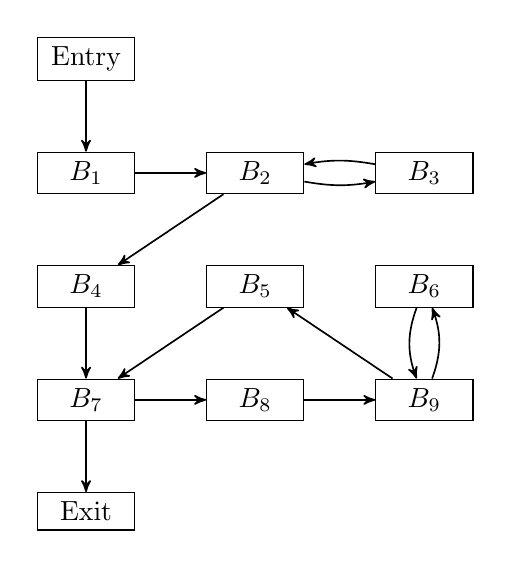
\begin{tikzpicture}
    \matrix[nodes={draw, rectangle, text width=1cm, align=center},
      row sep=9mm, column sep=9mm] {
        \node (B0) {Entry}; \\
        \node (B1) {$B_1$}; & \node (B2) {$B_2$}; & \node (B3) {$B_3$}; \\
        \node (B4) {$B_4$}; & \node (B5) {$B_5$}; & \node (B6) {$B_6$}; \\
        \node (B7) {$B_7$}; & \node (B8) {$B_8$}; & \node (B9) {$B_9$}; \\
        \node (BN) {Exit}; \\
    };

    \draw
      (B0) edge (B1)
      (B1) edge (B2)
      (B2) edge [bend right=10] (B3)
      (B2) edge (B4)
      (B3) edge [bend right=10] (B2)
      (B4) edge (B7)
      (B7) edge (BN)
      (B7) edge (B8)
      (B8) edge (B9)
      (B9) edge (B5)
      (B6) edge [bend right=20] (B9)
      (B9) edge [bend right=20] (B6)
      (B5) edge (B7)
    ;

\end{tikzpicture}
\end{center}
For the flow graph shown above,
identify the loops.
For each loop, give the loop entry.
%============================================================
\begin{framed}
Loop:

\begin{table}[h]
    \begin{tabular}{l | l}
        Basic Block                & Entries      \\
        \midrule
        $B_2$, $B_3$               & $B_2$        \\
        $B_5$, $B_7$, $B_8$, $B_9$ & $B_7$, $B_9$ \\
        $B_6$, $B_9$               & $B_9$        \\
    \end{tabular}
\end{table}

\end{framed}
%============================================================

\end{document}
